%-------------------------------------------------------------------------------
% Copyright (c) 2015-2016 University of Luxembourg.
% All rights reserved. This program and the accompanying materials
% are made available under the terms of the Eclipse Public License v1.0
% which accompanies this distribution, and is available at
% http://www.eclipse.org/legal/epl-v10.html
% 
% Contributors:
%     Alfredo Capozucca - initial writing
%     
%-------------------------------------------------------------------------------
%%%%%%%%%%%%%%%%%%%%%%%%%%%%%%%%%%%%%%%%%%%%%%%%%%
\PassOptionsToPackage{usenames,svgnames,table}{xcolor}
\documentclass[graybox,envcountchap,sectrefs]{./../lu.uni.lassy.excalibur.standard.report.libraries/styles/svmono}  
%%%%%%%%%%%%%%%%%%%%%%%%%%%%%%%%%%%%%%%%%%%%%%%%%%
%%% DO NOT CHANGE THE ORDER
\usepackage{./../lu.uni.lassy.excalibur.standard.report.libraries/styles/style-messir-common}
\usepackage{./../lu.uni.lassy.excalibur.standard.report.libraries/styles/style-messir-report-post}
\usepackage{breakurl}
%--------------------------------------------
 
% DOCUMENT BEGIN
%--------------------------------------------
\begin{document}
%-------------------------------------------------------------------------------
 
\newgeometry{textwidth=17cm,textheight=23.7cm} 
 
\definecolor{lightgray}{RGB}{201,201,201}
\definecolor{lightred}{RGB}{250,112,97}
\definecolor{lightgreen}{RGB}{179,250,140}

\definecolor{msrtextcl}{RGB}{0,0,0}
\definecolor{msrkeycl}{RGB}{127,0,85}
\definecolor{msrcmtcl}{RGB}{201,201,201}
\definecolor{keywordcolor}{RGB}{30,144,255}

\definecolor{aqua_blue}{RGB}{0,139,145}
\definecolor{dark_green}{RGB}{0,128,0}
\definecolor{dark_blue}{RGB}{45,45,138}

\definecolor{msrcolor01}{rgb}{0.96,0.59,0.48}
\definecolor{msrcolor02}{rgb}{1.00,0.97,0.60}
\definecolor{msrcolor03}{rgb}{0.51,0.79,0.61}
\definecolor{msrcolor04}{rgb}{0.43,0.81,0.96}
\definecolor{msrcolor05}{rgb}{0.52,0.58,0.79}
\definecolor{msrcolor06}{rgb}{0.96,0.61,0.76}
\definecolor{msrcolor07}{rgb}{0.98,0.68,0.51}
\definecolor{msrcolor08}{rgb}{0.77,0.88,0.61}
\definecolor{msrcolor09}{rgb}{0.49,0.66,0.85}
\definecolor{msrcolor10}{rgb}{0.96,0.60,0.62}
\definecolor{msrcolor11}{rgb}{0.64,0.83,0.61}
\definecolor{msrcolor12}{rgb}{0.63,0.53,0.75}
\definecolor{msrcolor13}{rgb}{0.99,0.78,0.54}
\definecolor{msrcolor14}{rgb}{0.53,0.51,0.74}
\definecolor{msrcolor15}{rgb}{0.48,0.80,0.79}
\definecolor{msrcolor16}{rgb}{0.74,0.55,0.75}
\definecolor{msrcolor17}{rgb}{0.90,0.79,0.08}
\definecolor{msrcolor18}{rgb}{1.00,1.00,0.00}
\definecolor{msrcolor19}{rgb}{1.00,0.00,0.50}

\definecolor{sepcolor000000}{rgb}{0, 0, 0}
\definecolor{sepcolor101010}{rgb}{0.10, 0.10, 0.10}
\definecolor{sepcolor202020}{rgb}{0.20, 0.20, 0.20}
\definecolor{sepcolor303030}{rgb}{0.30, 0.30, 0.30}
\definecolor{sepcolor404040}{rgb}{0.10, 0.10, 0.10}
\definecolor{sepcolor505050}{rgb}{0,1,.5}
\definecolor{sepcolor907908}{rgb}{0,1,.5}

\definecolor{sepregioncolor01}{rgb}{0.00,0.66,0.00}
\definecolor{sepregioncolor02}{rgb}{1.00,1.00,0.00}
\definecolor{sepregioncolor03}{rgb}{1.00,0.97,0.60}
\definecolor{sepregioncolor04}{rgb}{0.64,0.83,0.61}
\definecolor{sepregioncolor05}{rgb}{0.95,0.36,0.00}
\definecolor{sepregioncolor06}{rgb}{0.90,0.79,0.08}
\definecolor{sepregioncolor07}{rgb}{0.63,0.53,0.75}
\definecolor{sepregioncolor08}{rgb}{0.99,0.78,0.54}
\definecolor{sepregioncolor09}{rgb}{0.96,0.61,0.76}
\definecolor{sepregioncolor10}{rgb}{1.00,0.00,0.50}

\colorlet{msrcolorbrown}{red!40!black!80}


% Messir General
%----------------------------------------------------------

% quotePosition + quoteWidth + quotefillColor + quoteElement + quotedElement + allImageScale
\newcommand{\msrcallouted}[6]{
\scalebox{#1}{\parbox{\linewidth}{
  \begin{tikzpicture}
      \node [rectangle callout,callout relative pointer={#4},text width=#5,fill=#6,rounded corners] (tmpcall) at (0,0) {#3};
      \node at (tmpcall.pointer){#2};
  \end{tikzpicture}
}}
}

% Vresion wihtout scaling the quoted text
\pgfkeys{%
    /calloutquote/.cd,
    width/.code                   =  {\def\calloutquotewidth{#1}},
    position/.code                =  {\def\calloutquotepos{#1}}, 
    author/.code                  =  {\def\calloutquoteauthor{#1}},
    /calloutquote/.unknown/.code   =  {\let\searchname=\pgfkeyscurrentname
                                 \pgfkeysalso{\searchname/.try=#1,
    /tikz/\searchname/.retry=#1},\pgfkeysalso{\searchname/.try=#1,
                                  /pgf/\searchname/.retry=#1}}
                            }  

\newcommand\calloutquote[2][]{%
  \pgfqkeys{/calloutquote}{#1}
  \node [rectangle callout,callout relative pointer={\calloutquotepos},text width=\calloutquotewidth,/calloutquote/.cd,#1] (tmpcall) at (0,0) {#2};
  \node at (tmpcall.pointer){\calloutquoteauthor};    
}  
%----------------------------------------------------------
\newcommand{\msrTalkRD}[6]{
\freeblock{5}{#1}{#2}{
\begin{figure}
  \centering
  \includegraphics[width=#5]{images/various/descartes.pdf} 
\end{figure}
}
\freeblock{5}{#3}{#4}{
\scriptsize
\textit{#6}
}
}
\newcommand{\msrTalkGB}[6]{
\freeblock{5}{#1}{#2}{
\begin{figure}
  \centering
  \includegraphics[width=#5]{images/various/graham-bell.pdf} 
\end{figure}
}
\freeblock{5}{#3}{#4}{
\scriptsize
\textit{#6}
}
}
%----------------------------------------------------------

\newcommand{\msrQuestionSlide}[1]{
\begin{frame}[fragile]
\freeblock{5}{1}{4}{
\begin{figure}
  \centering
  \includegraphics[width=3cm]{images/various/3d-man-question-sit.pdf}
\end{figure}
}
\freeblock{10}{5}{3}{
\Large
\msrtxtclb{red}{\textit{#1}}
}
\end{frame}
}

%%%%%%%%%%%%%%%%%%%%%%%%%%%%%%%%%%%%%%%%%%%%%%%%%%

\DeclareRobustCommand{\msrfigure}[4]{
\begin{figure}[htbp]
%\centering
\scalebox{#1}{
{\begin{minipage}[c]{\linewidth}
\centering
#2
\end{minipage}
}}
\ifthenelse{\equal{#4}{}}
             {}
             {\caption{#4}}
\label{#3}
\end{figure}
}

\newcommand{\semitransp}[2][30]{\color{fg!#1}#2}
\newcommand*{\msrtechfont}{\fontfamily{ptm}\selectfont}

\DeclareRobustCommand{\msruml}{{\msrtechfont UML}~}
\DeclareRobustCommand{\msrocl}{{\msrtechfont OCL}~}
\DeclareRobustCommand{\msromg}{{\msrtechfont OMG}~}
\DeclareRobustCommand{\msrxtext}{{\msrtechfont Xtext}~}
\DeclareRobustCommand{\msremf}{{\msrtechfont EMF}~}
\DeclareRobustCommand{\msrcm}{\msrcode{{Concept Model}}~}

\DeclareRobustCommand{\msrapache}{{\msrtechfont Apache}~}
\DeclareRobustCommand{\msratlassian}{{\msrtechfont Atlassian}~}
\DeclareRobustCommand{\msrbamboo}{{\msrtechfont Bamboo}~}
\DeclareRobustCommand{\msrconfluence}{{\msrtechfont Confluence}~}
\DeclareRobustCommand{\msreclemma}{{\msrtechfont EclEmma}~}
\DeclareRobustCommand{\msreclipse}{{\msrtechfont Eclipse}~}
\DeclareRobustCommand{\msrsql}{{\msrtechfont SQL}~}
\DeclareRobustCommand{\msrjava}{{\msrtechfont Java}~}
\DeclareRobustCommand{\msrjavafx}{{\msrtechfont JavaFx}~}
\DeclareRobustCommand{\msrjira}{{\msrtechfont JIRA}~}
\DeclareRobustCommand{\msrjunit}{{\msrtechfont JUnit}~}
\DeclareRobustCommand{\msrlatex}{{\msrtechfont Latex}~}
\DeclareRobustCommand{\msrmaven}{{\msrtechfont Maven}~}
\DeclareRobustCommand{\msrmysql}{{\msrtechfont MySQL}~}
\DeclareRobustCommand{\msrocl}{{\msrtechfont OCL}~}
\DeclareRobustCommand{\msrpdf}{{\msrtechfont PDF}~} 
\DeclareRobustCommand{\msrsirius}{{\msrtechfont Sirius}~} 
\DeclareRobustCommand{\msrsvn}{{\msrtechfont SubVersioN}~}
\DeclareRobustCommand{\msrswtbot}{{\msrtechfont SWTbot}~}
\DeclareRobustCommand{\msrxtext}{{\msrtechfont Xtext}~} 

 
\DeclareRobustCommand{\msrmessirmeth}{{\msrmessir}~methodology~}
\newcommand{\msrglsstyle}[1]{\emph{#1}}
\DeclareRobustCommand{\msrucname}[1]{\msrcode{\underline{#1}}}

% Verify macro since creates .toc errors
%\DeclareRobustCommand{\msrcode}[1]{{\normalfont\fontfamily{pcrr}\selectfont #1}}
%\DeclareRobustCommand{\msrcode}[1]{{\normalfont\fontfamily{cmvtt}\selectfont #1}}
\DeclareRobustCommand{\msrcode}[1]{{\protect\ \ttfamily \hyphenchar\font=`\- #1}}

% Messir Lexique
\DeclareRobustCommand{\msrbool}{\msrcode{{\emph Boolean}}~}
\DeclareRobustCommand{\msrint}{\msrcode{{\emph Integer}}~}
\DeclareRobustCommand{\msrreal}{\msrcode{{\emph Real}}~}
\DeclareRobustCommand{\msrstring}{\msrcode{{\emph String}}~}
\DeclareRobustCommand{\msrenum}{\msrcode{{\emph enumeration}}~}
\DeclareRobustCommand{\msrenums}{\msrcode{{\emph enumerations}}~}

% Messir Analysis
\DeclareRobustCommand{\msrsysop}{\emph{system operation}}
\DeclareRobustCommand{\msrsysops}{\emph{system operations}}
\DeclareRobustCommand{\msrsysintpro}{\emph{system interaction protocol}}
\DeclareRobustCommand{\msrbhvmd}{\emph{system operation}}

\newcommand{\msrt}[1]{\textuncl{#1}~}

\DeclareRobustCommand{\msrfont}[1]{\textuncl{#1}}
\DeclareRobustCommand{\msrfontb}[1]{\msrfont{\textbf{#1}}}
\DeclareRobustCommand{\msrfontcl}[1]{\msrfont{{\color{MediumPurple}#1}}}
\DeclareRobustCommand{\msrfontclb}[1]{{\msrfontcl{\textbf{#1}}}}

\DeclareRobustCommand{\msrcl}[1]{{\color{MediumPurple}#1}~}
\DeclareRobustCommand{\msrclb}[1]{{\msrcl{\textbf{#1}}}}

\DeclareRobustCommand{\msrmessir}{\msrfont{Messir}~}
\DeclareRobustCommand{\msrmessirb}{\msrfont{\textbf{Messir}}}
\DeclareRobustCommand{\msrmessircl}{{\color{MediumPurple}\msrmessir}}
\DeclareRobustCommand{\msrmessirclb}{{\color{MediumPurple}\msrmessirb}}

\DeclareRobustCommand{\msrexcalibur}{{\unclfamily Excalibur}~}
\DeclareRobustCommand{\msrexcaliburb}{\msrfont{\textbf{\msrexcalibur}}}
\DeclareRobustCommand{\msrexcaliburcl}{\msrfontcl{\msrexcalibur}}
\DeclareRobustCommand{\msrexcaliburclb}{\msrfontclb{\msrexcalibur}}

\DeclareRobustCommand{\msrmessim}{\msrfont{MesSim}}
\DeclareRobustCommand{\msrmessimb}{\msrfontb{MesSim}}
\DeclareRobustCommand{\msrmessimcl}{\msrfontcl{MesSim}}
\DeclareRobustCommand{\msrmessimclb}{\msrfontclb{MesSim}}

\DeclareRobustCommand{\msrmessam}{\msrfont{MesSam}}
\DeclareRobustCommand{\msrmessamb}{\msrfontb{MesSam}}
\DeclareRobustCommand{\msrmessamcl}{\msrfontcl{MesSam}}
\DeclareRobustCommand{\msrmessamclb}{\msrfontclb{MesSam}}

\DeclareRobustCommand{\msrmevop}{\msrfont{MevoP}~}
\DeclareRobustCommand{\msrmevopb}{\msrfontb{MevoP}~}
\DeclareRobustCommand{\msrmevopcl}{\msrfontcl{MevoP}~}
\DeclareRobustCommand{\msrmevopclb}{\msrfontclb{MevoP}~}

\DeclareRobustCommand{\msrmessep}{\msrfont{Messep}~}
\DeclareRobustCommand{\msrmessepb}{\msrfontb{Messep}~}
\DeclareRobustCommand{\msrmessepcl}{\msrfontcl{Messep}~}
\DeclareRobustCommand{\msrmessepclb}{\msrfontclb{Messep}~}

\DeclareRobustCommand{\msrmessee}{\msrfont{MesSEE}~}
\DeclareRobustCommand{\msrmesseeb}{\msrfontb{MesSEE}~}
\DeclareRobustCommand{\msrmesseecl}{\msrfontcl{MesSEE}~}
\DeclareRobustCommand{\msrmesseeclb}{\msrfontclb{MesSEE}~}

\DeclareRobustCommand{\msrprolog}{{\msrtechfont Prolog}}
\DeclareRobustCommand{\msrmessimb}{\textbf{\msrmessim}}
\DeclareRobustCommand{\msrprologcl}{\textcolor{red}{\msrprolog}}
\DeclareRobustCommand{\msrprologclb}{\textbf{\msrprologcl}}

\DeclareRobustCommand{\msrmcl}{{\footnotesize \msrfont{mcl}}}
\DeclareRobustCommand{\msrmclb}{\msrfontb{\msrmcl}}
\DeclareRobustCommand{\msrmclclb}{\msrfontcl{\msrmclb}}
\DeclareRobustCommand{\msrmclcl}{\msrfontcl{\msrmcl}}

\DeclareRobustCommand{\msrmcltt}{\protect\ \msrmessir Constraint Language~}
\DeclareRobustCommand{\msrmessimtt}{\protect\ \msrmessir Simulator~}
\DeclareRobustCommand{\msrmessamtt}{\protect\ \msrmessir Abstract Machine~}

\DeclareRobustCommand{\generic}{\textbf{\textit{{\color{MediumPurple}generic}}}~} 
\DeclareRobustCommand{\msrhelloworld}{\textbf{\textit{{\color{MediumPurple}HelloWorld}}}~}
\DeclareRobustCommand{\msricrash}{\textbf{\textit{{\color{MediumPurple}iCrash}}}~} 
\DeclareRobustCommand{\msricrashmini}{\textbf{\textit{{\color{MediumPurple}iCrashMini}}}~}  

\DeclareRobustCommand{\msrtxtcl}[2]{{\color{#1}#2}}
\DeclareRobustCommand{\msrtxtclb}[2]{\msrtxtcl{#1}{\textbf{#2}}}


%---------TABLES TEMPLATE--------------

%\rowcolors{2}{gray!20}{}

\newcounter{itemtable}


\newenvironment{usecase}{\begin{longtable}{|p{0.10\textwidth}
p{0.90\textwidth}|} \hline} {\hline \end{longtable}}


\newenvironment{usecaseinstance}{\begin{longtable}{|p{0.05\textwidth}
p{0.95\textwidth}|} \hline}
{\hline \end{longtable}}


\newenvironment{actortable}{
\begin{longtable}{|p{0.10\textwidth} p{0.90\textwidth}|}
\hline \hline}
{\hline \end{longtable}}


\newenvironment{datadictionary}{
\begin{longtable}{|p{0.15\textwidth} p{0.85\textwidth}|}
\hline \hline}
{\hline \end{longtable}}


\newenvironment{associationtypes}{
\begin{longtable}{|p{0.15\textwidth} p{0.85\textwidth}|}
\hline \hline}
{\hline \end{longtable}}


\newenvironment{operationmodel}{
\setcounter{itemtable}{0}
\begin{longtable}{|p{0.10\textwidth} p{0.90\textwidth}|}
\hline \hline}
{\hline \end{longtable}}


\newenvironment{teststepmodel}{
\setcounter{itemtable}{0}
\begin{longtable}{|p{0.10\textwidth}|p{0.90\textwidth}|}
\hline}
{\hline \end{longtable}}


\newcommand*{\myfont}{\fontfamily{phv}\selectfont}


\newcommand\addheading[1]{
\hline
%\multicolumn{2}{|l|}{\cellcolor[gray]{0.9} \textbf{#1}} \\
\multicolumn{2}{|l|}{\textbf{\scshape #1}} \\
\hline \hline
\endfirsthead

\multicolumn{2}{@{}l}{\myfont{\bfseries\itshape{\ldots #1 table
continuation}}}\\
%\hline \hline
%\multicolumn{2}{|l|}{\cellcolor[gray]{0.9} \textbf{#1}}\\
%\hline \hline
\endhead % all the lines above this will be repeated on every page

%\hline \hline
\multicolumn{2}{r@{}}{\myfont{\bfseries\itshape{continues in next page
\ldots}}}\\
\endfoot

\hline
\endlastfoot}

%\multicolumn{2}{|l|}{\cellcolor[gray]{0.8}
\newcommand\addrowheading[1]{
\hline \hline
\multicolumn{2}{|l|}{
  \setcounter{itemtable}{0}
  \textbf{\itshape #1}}\\
\hline \hline
}


\newcommand\addsinglerow[1]{
\multicolumn{2}{|l|}{\begin{minipage}[t][][t]{1.0\textwidth}
#1 \end{minipage}} \\
%\hline
}


\newcommand\addsingletwocolumnrow[2]{
{\itshape #1} & #2 \\
%\hline
}


\newcommand\adddoublerow[2]{
\hline \hline
\multicolumn{2}{|l|}{\begin{minipage}[t][][t]{1.0\textwidth}
\textbf{\itshape #1} \end{minipage}} \\
\multicolumn{2}{|l|}{\begin{minipage}[t][][t]{1.0\textwidth}
#2 \end{minipage}} \\
\hline
}


\newcommand\adddoubletwocolumnrow[3]{
#1 & \textbf{#2} \\
& #3 \\
%\hline
}


\newcommand\addnumberedsinglerow[2]{
\stepcounter{itemtable}
\text{#1 \theitemtable} & #2 \\
%\hline
}


\newcommand\addnumbereddoublerow[3]{
\stepcounter{itemtable}
\text{#1 \theitemtable} & \textbf{#2} \\
       & #3 \\
%\hline
}



\newcommand\addalphanumberedsinglerow[2]{
\stepcounter{itemtable}
\text{#1 \alph{itemtable}} & #2 \\
%\hline
}


\newcommand\addalphanumbereddoublerow[3]{
\stepcounter{itemtable}
\text{#1 \alph{itemtable}} & \textbf{#2} \\
       & #3 \\
%\hline
}

%%%%%%%%%%%%%%%%%%%%%%%%%%%%%%%%%%%%%%%%%%%%%%%%%%%%%%%%%%%%%%%%%%%%%%%%%%%%
%%%%%%%%%%%%%%%%%%%%%%%%%%%%%%%%%%%%%%%%%%%%%%%%%%%%%%%%%%%%%%%%%%%%%%%%%%%%

\lstdefinelanguage{MessirProlog}{
morekeywords=[1]{msrNav,msrop,:-},
morekeywords=[2]{msrVar},
morekeywords=[3]{msrTrue,msrFalse,true,false,msrIsNew,msrIsKilled,msrForAll,msrExists,msrSelect,msrReject,msrClose,msrAny,msrIsEmpty,msrSize,msmAtPre,msmAtPost,msrColEq,msrColSubtract,msrCount,msrExcludes,msrExcludesAll,msrIncludes,msrIncludesAll,msrSum,msrProd,msrIncluding,msrExcluding,msrIntersection,msrUnion,msrAsSet,msrOne},
morekeywords=[3]{rnSystem,rnActor,rnSystem,rnInterfaceIN,rnInterfaceOUT,ptBoolean,ptReal,ptString,ptInteger,preProtocol,preFunctional,postProtocol,postFunctional,init},
morekeywords=[4]{Self},
sensitive=true,
morestring=[b]{"},
comment=[s]{/*}{*/},
morecomment=[l]//
}[keywords,comments,strings]%
 
\lstdefinestyle{MessirPrologStyle} { 
language=MessirProlog,
extendedchars=true,
basicstyle=\ttfamily,
%keywordstyle=\color{blue}\bfseries,
keywordstyle=[1]\color{blue}\bfseries,
keywordstyle=[2]\color{red},
keywordstyle=[3]\color{msrcolor12}\bfseries,
keywordstyle=[4]\color{msrcolor09}\bfseries,
stringstyle=\color{msrtextcl},
commentstyle=\color{msrcmtcl},
breakatwhitespace=false,
tabsize=1,
literate={\ \ }{{\ }}1,
breaklines=true,
emptylines=1,
numbers=left,
numberstyle=\tiny\color{blue}, 
firstnumber=auto,
stepnumber=1,
numbersep=0pt, 
showspaces=false,
showlines=false,
numberfirstline=true,
showstringspaces=false
showtabs=false,
includerangemarker=true
}



\lstdefinestyle{MessirStyle} { 
language=Messir,
extendedchars=true,
basicstyle=\ttfamily,
keywordstyle=\color{msrkeycl}\bfseries,
stringstyle=\color{msrtextcl},
commentstyle=\color{msrcmtcl},
breakatwhitespace=false,
tabsize=1,
literate={\ \ }{{\ }}1,
breaklines=true,
emptylines=1,
numbers=left,
numberstyle=\tiny\bfseries\color{blue}, 
firstnumber=auto,
stepnumber=1,
numbersep=2pt, 
showspaces=false,
showlines=false,
numberfirstline=true,
showstringspaces=false
showtabs=false,
includerangemarker=true
}

\lstdefinelanguage{Messir}{
keywords={package,import,Concept,Model,Primary,Types,Secondary,state,class,
role,cardinality,extends,attribute,external,operation,primitive,
datatype,enum,constants,association,aggregation,composition,Environment,
actor,role,input,interface,output,Operation,external,link,preF,preP,postF,
postP,ocl,Test,test,case,order,step,prolog},
morekeywords=[1]{self,let,in,true,false,result},
morekeywords=[2]{name,attributes,associatoinEnds,operations,%
      supertypes,allSupertypes,allInstances,oclIsKindOf,oclIsTypeOf,%
      oclAsType,oclInState,oclIsNew,evaluationType,abs,floor,round,max,%
      min,div,mod,size,concat,toUpper,toLower,substring,includes,%
      excludes,count,includesAll,exludesAll,isEmpty,notEmpty,sum,%
      exists,forAll,isUnique,sortedBy,iterate,union,intersection,%
      including,excluding,symmetricDifference,select,reject,collect,%
      asSequence,asBag,asSequence,asSet,append,prepend,subSequence,at,%
      first,last,true,false,isQuery,context,pre,inv,post},
    morekeywords=[3]{and,equiv,exit,impl,not,or},%
    morekeywords=[4]{Boolean,Integer,Real,String,Set,Sequence,Bag,%
       OclType,OclAny,OclExpression,Enumeration,Collection},%
    morekeywords=[5]{Use,use,system,Case,Model,related,instance,primary,secondary,oracle,value,constraint,message,parameter,value,truth,protocol,functional,variables,values,results,subfunction,usergoal,summary,executes,sends,to,reuse,received,from,ordering,if,then,else,endif,self,^},
    morekeywords=[6]{executed,instanceof,returned,steps,active,passive,proactive,constraints,multiple},
    morekeywords=[7]{@Actor,@actorDeclaration,@actorSpecification,@additionalInformation,@attribute,@caption,@colOperation,@constraint,@description,@endActorsDeclaration,@endActorsSpecification,@endAttributes,@endColOperations,@endConstraints,@endInputEvents,@endInputParametersDeclaration,@endInputParametersSpecification,@endInstanceOracleOutputParameters,@endInstanceTestReceivedMessages,@endOperations,@endOracleConstraints,@endOracleOutputParametersSpecification,@endOracleReceivedMessagesSpecification,@endOracleValues,@endOracleVariables,@endOutputEvents,@endOutputParametersDeclaration,@endOutputParametersSpecification,@endParameters,@endPostConditions,@endPostF,@endPostP,@endPreConditions,@endPreF,@endPreP,@endProtocolConditions,@endRemarks,@endStepOrderingConstraints,@endVariables,@endVariableValues,@example,@inputEvent,@inputParameterDeclaration,@inputParameterSpecification,@Instance,@instanceOracleOutputParameter,@instanceTestReceivedMessage,@level,@model,@number,@Operation,@oracleConstraint,@oracleOutputParameterSpecification,@oracleReceivedMessageSpecification,@oracleSpecification,@oracleTruthValue,@oracleValue,@oracleVariable,@orientation,@outputEvent,@parameter,@postCondition,@postF,@postP,@preCondition,@preF,@preP,@Primary,@protocolCondition,@remark,@return,@scale,@Secondary,@stepOrderingConstraint,@sublevel,@Test,@testResultPostFunctional,@testResultPreFunctional,@testResultPreProcotol,@testSentMessage,@testSentMessageValue,@Use,@variable,@variableValue,@view,@pre,@post},
    morekeywords=[8]{@@Use,@@Instance,@@Primary,@@Secondary,@@Actor,@@Operation,@@Test,@@Instance,@@view,@operation},
sensitive=true,
morestring=[b]{"},
comment=[s]{/*}{*/},
morecomment=[l]//
%alsodigit={.}
}[keywords,comments,strings]%
%%%%%%%%%%%%%%%%%%%%%%%%%%%%%%%%%%%%%%%%%%%%%%%%%%%%%%%%%%%%%%%%%%%%%%%%%%%%
%%%%%%%%%%%%%%%%%%%%%%%%%%%%%%%%%%%%%%%%%%%%%%%%%%%%%%%%%%%%%%%%%%%%%%%%%%%%

%%%%%%%%%%%%%%%%%%%%%%%%%%%%%%%%%%%%%%%%%%%%%%%%%%%%%%%%%%%%%%%%%
%%%%%%%%%%%%%%      150506    %%%%%%%%%%%%%%%%%%%%%%%%%%%%%%%%%%%
%%%%%%%%%%%%%%%%%%%%%%%%%%%%%%%%%%%%%%%%%%%%%%%%%%%%%%%%%%%%%%%%%

\DeclareRobustCommand{\msrsee}{software engineering environment~}

\newcommand\freeblock[4]{%
\begin{textblock}{#1}(#2,#3)
\begin{minipage}{\textwidth}
\setlength{\parindent}{0pt}%
\setlength{\parskip}{0.1cm}%
#4
\end{minipage}
\end{textblock}
}
 
\newcommand\addheadingPS[4]{
\hline
\multicolumn{2}{|l|}{\textbf{\scshape Process Step}} \\
\hline
\multicolumn{2}{|l|}{Phase: \msrclb{#1} - Iteration: \msrclb{#2} - Step: \msrclb{#3}}\\
\hline
\multicolumn{2}{|l|}{Name: \msrclb{#4}}\\
\hline \hline
\endfirsthead 

\multicolumn{2}{@{}l}{\myfont{\bfseries\itshape{\ldots #1 table
continuation}}}\\
\endhead % all the lines above this will be repeated on every page

\multicolumn{2}{r@{}}{\myfont{\bfseries\itshape{continues in next page
\ldots}}}\\
\endfoot

\hline
\endlastfoot}

\newenvironment{processsteptable}{
\setcounter{itemtable}{0}
\begin{longtable}{|p{0.10\textwidth}|p{0.90\textwidth}|}
\hline}
{\hline \end{longtable}
}

%%%%%%%%%%%%%%%%%%%%%%%%%%%%%%%%%%%%%%%%%%%%%%%%%%
\newcommand{\mybox}[2]{\par\noindent\colorbox{#1}
{\parbox{\dimexpr\textwidth-2\fboxsep\relax}{#2}}}

%for time line tables
\newcommand\ytl[5]{
\parbox[b]{8em}{\hfill{\color{#2}\bfseries\sffamily #3}~$\cdots\cdots$~}\makebox[0pt][c]{$\bullet$}\vrule\quad \parbox[c]{\textwidth}{\vspace{#1pt}\color{#4}\raggedright\sffamily #5\\[7pt]}\\[-3pt]}

% For setting item spacing
% ex: {\setlistspacing{2}{2ex} \begin{frame} \ldots \end{frame}}
\makeatletter
\newcommand{\setlistspacing}[2]{\def\@ld{#1}\expandafter\def\csname
@list\romannumeral\@ld \endcsname{\leftmargin\csname
leftmargin\romannumeral\@ld \endcsname
              \topsep    #2
              \parsep    0\p@   \@plus\p@
              \itemsep   #2}}
\makeatother




% ***************************************
% test-case schema template
\newenvironment{lyxlist}[1]
  {\begin{list}{}
    {\settowidth{\labelwidth}{#1}
      \setlength{\leftmargin}{\labelwidth}
      \addtolength{\leftmargin}{\labelsep}
      \renewcommand{\makelabel}[1]{##1\hfil}}
      \setlength{\itemsep}{0ex}
      \addtolength{\baselineskip}{-5pt}
			\setlength{\parskip}{0pt}
			\setlength{\parsep}{0pt}}
  {\end{list}}
  
  
  \def\Remark{\noindent\textit{Remark : }}
  
  \DeclareRobustCommand{\mysystemname}{\textbf{\textit{{\color{MediumPurple}MySystem
  (v1.0)}}}~}
  
%GLOSSARY

\printglossaries
\newpage  

%TITLE
%******************************************
\title{
\begin{tabular}{|>{\centering\arraybackslash\hspace{0pt}}p{16cm}|}
\hline
\textbf{HighwayToSafety}\\ \\
	\textbf{\msrmessir User Manual}\\
	\textbf{ - v 1.0.3 - }\\
	\textbf{\large Based on IEEE Std 1063-2001 \cite{IEEE-2001-userdocumentation}}\\
\hline 
\end{tabular}
\vspace{2cm}}
 
%******************************************
\author{
\begin{tabular}{l}
		Scholer Tom\\
		Mok Zhi Kin\\
		\\Group 09 - University of Luxembourg\\
\end{tabular}}

\date{\today~-~\currenttime}
%****************************************************


\maketitle
\newpage

%TOC
\setcounter{tocdepth}{2}
\addtocounter{secnumdepth}{2}
\tableofcontents
\newpage

%TOF
\listoffigures
\newpage

% No requiered by the standard
%TOL
%\lstlistoflistings
%\newpage

%DOCUMENT STRUCTURE

% General Information
\chapter{Product information}
%Reducing the spacing from the title
\vspace{-6em}

\newglossaryentry{PdtName}{name={HighwayToSafety}, desciption={Name of our
Crisis Management System}}

\section{Identification}
%Include precise information of the software product like identification name
%(that you can include in the \gls{PdtName}), list of parts that compose it
%(indicating identification numbers for each part).
%pecify the applicable operating environment(s), including version(s) of
% hardware, communications, and operating system(s).
<\gls{PdtName} - XN1000> is a web application meant to be used on any internet
browsers on any platform and an adapted version is also included for any iPad
with a version of iOS later than iOS 7.

\section{Copyright}
Copyright \copyright \ 2016 by University of Luxembourg. All rights reserved.

\section{Trademark notices}
HighwayToSafety \circledR, the HighwayToSafety Logo and related trade dress are
trademarks or registered trademarks of the University of Luxembourg and/or its
affiliates, and may not be used without written permission. All other trademarks
are the property of their respective owners. University of Luxembourg is not
associated with any product or vendor mentioned in this user-manual.

\section{Restrictions}
No part of this manual, including the software described in it, may be
reproduced, transmitted, transcribed, stored in a retrieval system or translated
into any language in any form or by any means, except by the purchaser for
backup purposes, without prior written permission of the University of
Luxembourg.

\section{Warranties}
University of Luxembourg warrants that for a period of two years from the date
of purchase that the Software conforms to it's published specifications. This
limited warranty extends only to Customer as the original licensee. In case of
malfunctioning and not providing the mentioned specification, University of
Luxembourg offers to refund or replace the software to their customers. In no
event does University of Luxembourg warrant that the Software is error free or
that Customers will be able to operate the Software without problems or
interruptions. This warranty does not apply if the software (a) has been
altered, except by University of Luxembourg, (b) has not been installed,
operated, repaired, or maintained in accordance with instructions supplied by
University of Luxembourg, (c) has been subjected to abnormal physical or
electrical stress, misuse, negligence, or accident, or (d) is used in
ultrahazardous activities.

\section{Contractual obligations}
All information, written or oral, that the customer discloses or makes available
to the developer through any means of communication is confidential.
University of Luxembourg performs services for the customer such as support and
maintain the software during the validity of the warranty.
University of Luxembourg will be responsible for conducting all activities
required to install the software at the customer's premises.
The customer will have 10 days following the date of installation to test the
software.
If University of Luxembourg fails to deliver the software with the desired
specifications, the customer shall detail in writing its reasons for rejection.
In that case, University of Luxembourg shall correct the software.

\section{Disclaimers}
University of Luxembourg reserves the right to revise this publication and to
make changes from time to time in the content hereof without obligation of the
University of Luxembourg to notify any person of such revision or changes.

\section{Contact}
In case of any problem or question the customer can visit our website:
https://uni.lu/highwaytosafety.                                                 
They can also reach our helpline during business hours: 00352 11 12 34 56.      
Or send an email to: highwaytosafety.help@uni.lu
\newpage

% Introduction
\chapter{Introduction}
\label{chap:introduction}

\section{Scope}
This User Manual explains how to install, configure and use HighwayToSafety. The
instructions here apply to version 1.0 of HighwayToSafety.
This document does not provide any information on how to perform changes like
adding functionalities. It is not intended to provide information about
third-party software or devices.
It may be used with other first party support documantation
downloadable on our website www.uni.lu/highwaytosafety/support.
%Example: This document provides minimum acceptable information for knowing how
% to use the software system \mysystemname.
 
%Example: This document is not intended to provide information about how to
% connect, deploy, configure, or use any external device or
% third-party software system that is rqeuired for the correct funcitoning of
% \mysystemname.
%This document may be used with other documents provided by third-party
% companies to have an overall view and correct understanding of the environment
% and procedures where the software system \mysystemname is aimed to be deployed
% and run.
\section{Purpose}
This document provides information on when and how to use our software. It
describes the operation and performance of the HighwayToSafety software as used
by emergency offices and their associates.
\section{Intended audience}
This document is intended to serve as a guide for every user of the
HighwayToSafety software. It is used by different kinds of administrators, who
are guided in a step-by-step fashion to execute the different functionalities
provided by the software.
It is also used by different kinds of coordinators, who are shown how to
effectively use the software, without creating any confusions, and how to assure
a smooth operation.

\section{HighwayToSafety}
This software is intended to help organising and managing the
aftermath of an highway-car-crash as effectively as possible.
It assures the communication between the workforce, who are on the site of the
accident, and their colleagues who work at the emergency centrals. 


\subsection{Actors \& Functionalities}
In this section, you will find an overview of all the
\textbf{\emph{\glspl{actor}}} interacting with the software. The structure of
this section is such that for each actor, you will find a short introduction
followed by the main software functions that are offered to him.

\subsubsection{Emergency Central}
\subparagraph{Emergency Central Administrator}
Most likely a chief or someone with high autorities in the Emergency Central. His
job is to assign fellow colleagues as coordinators.

\subparagraph{Emergency Central Coordinator}
An Emergency Central Coordinator is an employee who has been given special rights
by the administrator. His job is:

\begin{enumerate}
\item To confirm the notifier's situation.
\item To register any useful information given by the notifier.
\item To check the incident's location with the notifier.
\item To submit the new event to the CMS when needed.
\item To send a dispatch message including the incident's location to the
incident's nearest Police Teams, Firemen Teams and/or Towing Service Vehicles.
\item To send a message to the News Company including the incident's location to
broadcast the traffic jam that it will cause.
\item To make sure the number of any requested Teams matches the number of Teams
on its way and/or on-site. If overloaded, than make sure as many as possible are
dispatched.
\item To have an overview over the events in case the on-site workers are
troubled or if they need more precise information on the dispatched teams.
\end{enumerate}



\subsubsection{Firemen}
\subparagraph{Firemen Administrator}
Most likely a chief or someone with high autorities in the Firemen Department.
His job is to assign fellow colleagues as coordinators.

\subparagraph{Firemen Coordinator}
A Firemen Coordinator is a Team Leader who has been given special
rights by the administrator. His job is:

\begin{enumerate}
\item To assemble his team as soon as possible when a dispatch request is
received.
\item To provide information on how long it takes to be on-site.
\item To call for backup if needed when on-site.
\item To eventually inform everyone (not just the Police) of any kind of
emergencies related to the incident.
\item To organise blockades of the highway and deviations.
\item To alert the Towing Service to clear the highway of the crashed cars.
\end{enumerate}

\subsubsection{Police}
\subparagraph{Police Administrator}
Most likely a chief or someone with high autorities in the Police Department.
His job is to assign fellow colleagues as coordinators.

\subparagraph{Police Coordinator}
A Police Coordinator is a Team Leader who has been given special
rights by the administrator. His job is:

\begin{enumerate}
\item To assemble his team as soon as possible when a dispatch request is
received.
\item To provide information on how long it takes to be on-site.
\item To call for backup if needed when on-site.
\item To eventually inform everyone (not just the Police) of any kind
of emergencies related to the incident.
\end{enumerate}


\subsubsection{Communication Company}
A Communication Company is a company who provides fixed and mobile voice
services like POST, TANGO, ORANGE, etc. Its job is to transfer any emergency
calls to the Emergency central for free and to provide the notifier's
coordinates via its network to the system.


\subsubsection{Activator}
An Activator is a logical representation of the active part of our CMS. It represents an
implicit stakeholder belonging to the system's environment that interacts with
our CMS autonomously without the need of external entity. It is usually time triggered
functionalities. Its job is to communicate the current time and date to the
system everytime an operation's processed.


\subsection{Operating environment}
%Brief overview of the infrastructure on which the software is deployed and
% used.
The department of Fire and Emergeny Services is a critical part of the State
Services that needs quick actions and communication in order to minimize the
casualties and inconveniences during emergencies such as car crash, school fire,
etc. \\\\
For the sake of a smooth execution of its tasks, it requires the
cooperation of several other infrastucture such as the Hospital departments
which are also greatly impacted during emergencies to take care of the injured
and a good communication service between these institutions would also be
required. \\\\
In our scenarios, it most likely also requires to have the cooperation of
the towing service to take care of the broken cars and the Highway maintenance
service to eventually seal off parts of the Highway.

\section{Document structure}  
%Information on how this document is organised and it is expected to be
%used. Recommendations on which members of the audience
%should consult which sections of the document, and explanations about the used
%notation (i.e. description of formats and conventions) must also be provided.
This user-manual is basically split into two parts. \\\\
The first two chapters are meant to introduce the user-manual. Any user should
have a look at these chapters to get a good overview of the manual. \\\\
The second part going from chapter 3 to chapter 5 are the more technical
part mostly composed of distinct procedures, operations or problems, meaning
that by reading the description of the concerned section, the user should be
able to identify whether it corresponds to their needs. As such, users would
mostly be looking for a procedure in chapter 3 corresponding to their functions
that bears resemblances to their own case and check out the section that
explain in details their part. Otherwise if they encounter any error messages or
problems of the system, they would need to check out chapter 5 for more
information.
Chapter 4 is mainly written for the purpose of understanding how the whole
system works together through different software operation hidden from the
users.






\newpage

% User guide
\chapter{Usage Guide}
\label{chap:usage_guide}
HighwayToSafety is a software designed for a lot of different users with a lot
of different interfaces. However, every user just needs to know how the
interface, that he is going to work with, functions. The coordinators of the
firemen and policemen for instance have to work with a very simple application.
It's easy to use because they eventually work with it on the site of the
accident, where it might be very noisy and chaotic.
The administrators and emergency central work with a little more complex
application, which allows them to manage and organise ressources such as human
ressources, equipment and vehicles.

This section is aimed at describing the general use of each actor by using
procedure descriptions. The description of the processes is organised in a way
to facilitate learning by presenting simpler, more common, or initial processes 
before more complex, less utilised, or subsequent processes.

\textbf{(including installation procedures)}.

 \cite{armour01usecase} \textbf{BUT its content must be as low level as possible with actual values}:
\vspace{0.5cm}
\hrule
\begin{lyxlist}{UC1}
\small{
\item [\textbf{Use~Case:}] ProcessMissionOne
\item [\textbf{Scope:}] Crisis Management System (\emph{CMS})
\item [\textbf{Primary Actor}:] Coordinator John
\item [\textbf{Secondary Actor}:] FirstAidWorker Bob,\\
                  ExternalResourceSystem (ERS)
\item [\textbf{Intention:}]The intention of the Coordinator is to process mission with ID equal to 1.
\item [\textbf{Level}:]Sub-functional level
\item [\textbf{Main~Success~Scenario}]:\\
1. \emph{John} instructs the \emph{CMS} to process a specific mission.\\
2. \emph{CMS} selects the internal worker \emph{Bob} to execute the mission.\\
3. \emph{CMS} instructs `\emph{Bob} to behave as \emph{FAW}.\\
4. \emph{Bob} informs to the \emph{CMS} of his arrival.\\
5. \emph{Bob} executes the mission.\\
6. \emph{Bob} informs to the \emph{CMS} the mission outcome.


\item [\textbf{Extensions}]:\\
2.a None internal worker can execute the mission.\\
\hspace*{0.5cm} 2.a.1 \emph{CMS} requests an external resource to \emph{ERS}.\\
\hspace*{0.5cm} 2.a.2 \emph{ERS} informs \emph{CMS} that the request can be processed.\\
\hspace*{1.4cm} Use case continues at step 3.

}

\end{lyxlist}
\hrule
\vspace{0.5cm}

\Remark{Graphical User Interfaces (GUIs)}: include GUIs screenshots to show the
different stages of the process while its is performed by the actor.



\section{Actors common procedures}
Common procedures to several actors are grouped in this section to avoid
redundancy.

\subsection{suGlobalManagementOfEvent}

\begin{lyxlist}{UC1}
\small{
\item [\textbf{Use~Case:}] suGlobalManagementOfEvent
\item [\textbf{Scope:}] Enterprise level
\item [\textbf{Primary Actor}:] Walter: Human Witness,\\ 
						        Camille: Central Coordinator,\\
								Fabio: Firemen Coordinator,\\
								Ted: Tow-truck driver,\\ 
								Polo: Police Coordinator
\item [\textbf{Secondary Actor}:] Orange: Communication Company
\item [\textbf{Intention:}] The intention of this procedure is to have a new
event\\ registered into the system and have all the required resources\\ arrive
at the accident’s location.
\item [\textbf{Level}:] Summary level
\item [\textbf{Main~Success~Scenario}]:
\begin{enumerate}
  \item Walter contacts by phone Camille at the Emergency Central.
  \item Camille sends a message to HTS(i.e. Highway to Safety) to request
  coordinates of Walter's phone number 00352 691 12 34 56.
  \item HTS sends a message to Orange to receive the coordinates of the user
  with phone number 00352 691 12 34 56.
  \item Orange sends coordinates of phone number 00352 661 123 123 to HTS.
  \item HTS sends Walter's coordinates to Camille.
  \item Camille asks the system to create a new event associated to the crisis
  with the following information:
  \begin{enumerate}
  \item Walter (name)
  \item Witness (actor type)
  \item ``Highway carcrash with two cars involved'' (comment)
  \end{enumerate}
  \item HTS creates the new event with the information given by Camille and
  generates a new crisisID:1 to the event.
  \item HTS adds phone number and coordinates of phone number to the event 1.
  \item HTS sends a request to dispatch a team to the nearest, available Firemen
  Coordinator Fabio.
  \item HTS sends a request to dispatch a tow-truck to the nearest, available
  Tow-truck driver Ted.
  \item Fabio sends a message to HTS that his team is on its way to the
  accident’s location.
  \item Ted sends a message to HTS to refresh the map.
  \item Ted sends a message to HTS (``I will arrive in 30 minutes'').
  \item Ted sends a message to HTS that he is on his way to the accident’s
  location.
  \item Fabio sends a message to HTS that his team has arrived at the accident’s
  location.
  \item Fabio sends a message to HTS that they require a Police Team.
  \item HTS sends a request to dispatch a team to the Police Coordinator Polo.
  \item Polo sends to HTS that his team is on its way to the accidents
  location.
  \item Ted sends a message to HTS that he has arrived at the accident’s
  location.
  \item Polo sends a message to HTS that his team has arrived at the accident’s
  location.
\end{enumerate}
}
\end{lyxlist}



\begin{minipage}{0.72\textwidth}
\begin{figure}[H]
\caption{New Event window}
\includegraphics[width=1.0\textwidth]{GetLocation.eps}
\end{figure}
\end{minipage} \hfill
\begin{minipage}{0.23\textwidth}
\begin{itemize}
\item 1.By pressing the ``Get Location'' button the Camille asks the system to
get the location of the phone number of the witness.
\item 2. These fields are filled by Camille with the corresponding
information as described in step 6 of the main success scenario.
\end{itemize}
\end{minipage}

\begin{minipage}{0.72\textwidth}
\begin{figure}[H]
\caption{Change Status GUI}
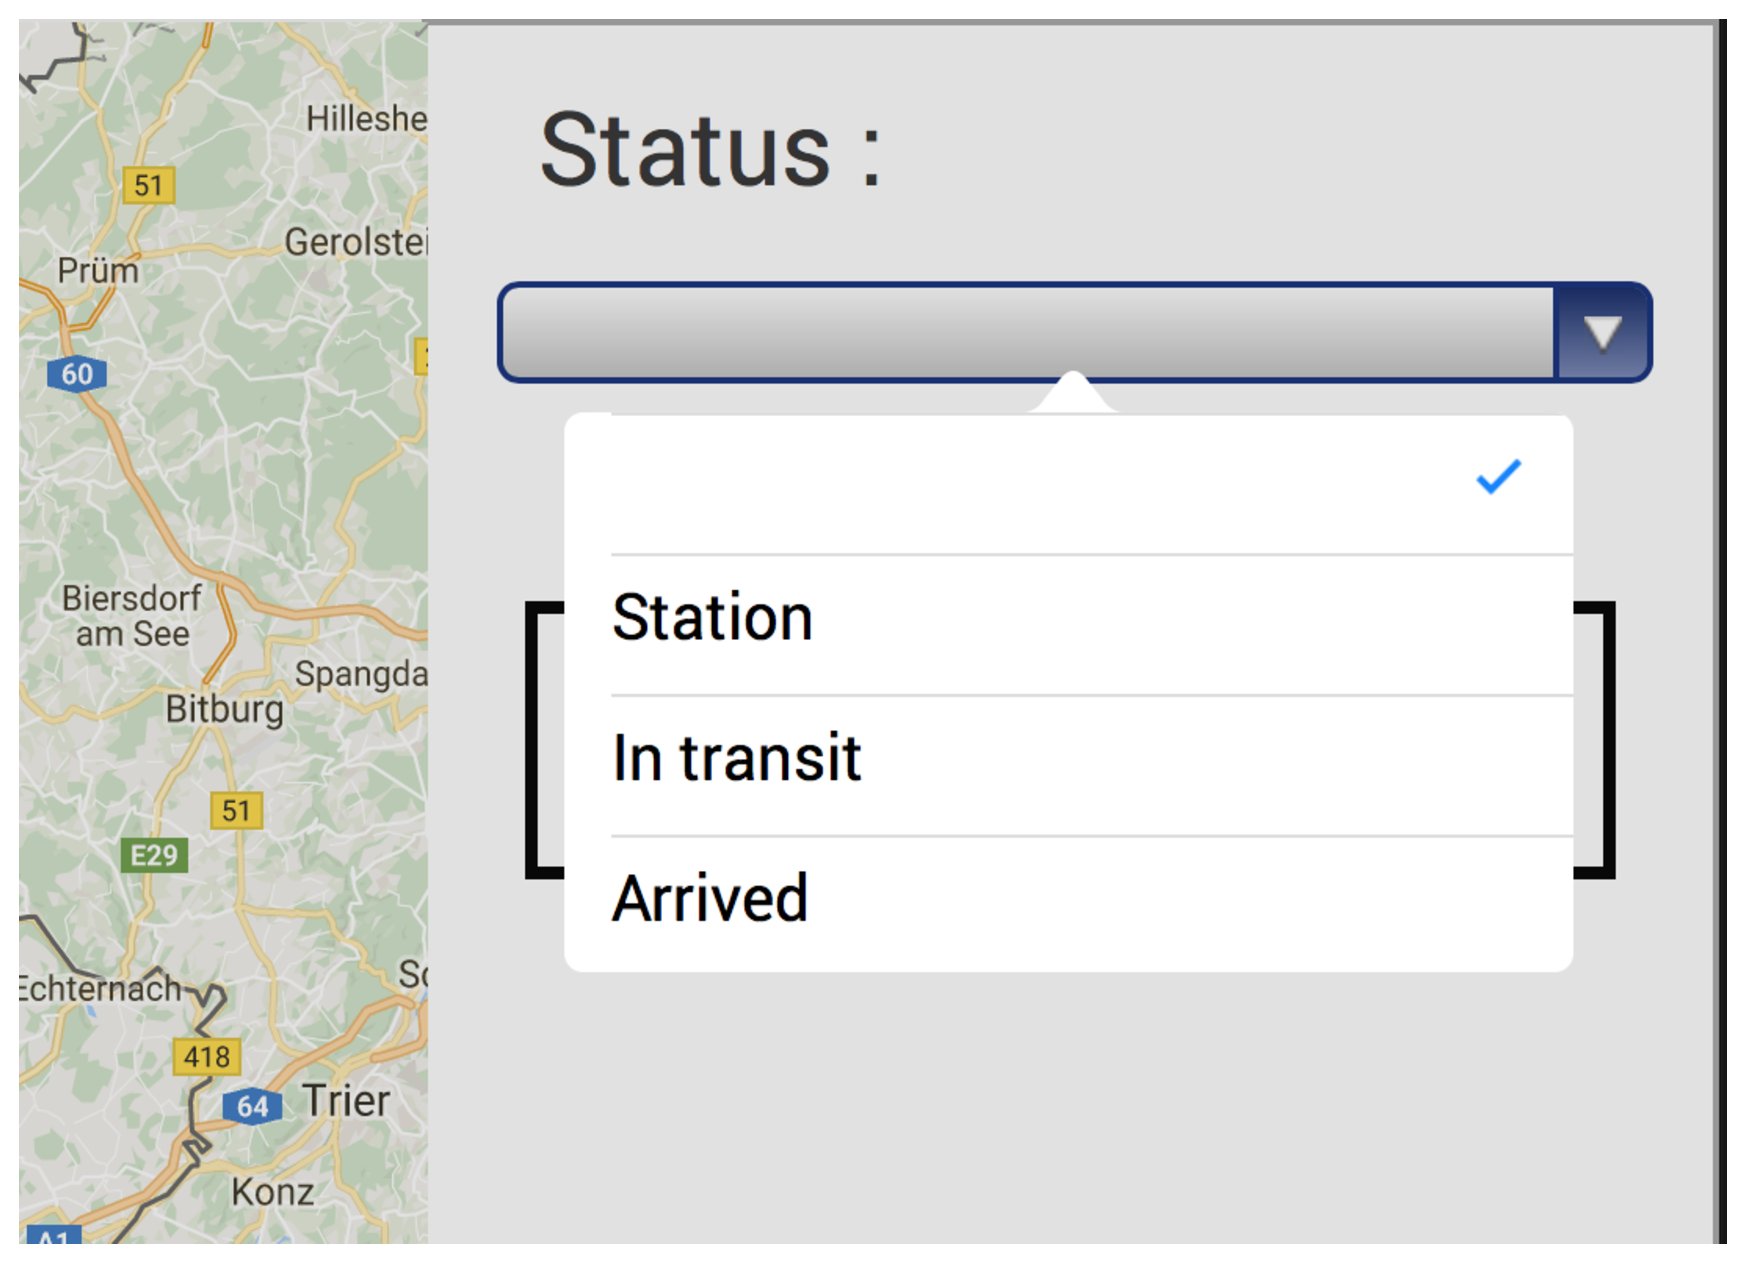
\includegraphics[width=1.0\textwidth]{Ipad_status.eps}
\end{figure}
\end{minipage} \hfill
\begin{minipage}{0.23\textwidth}
\begin{itemize}
\item As described in steps 11, 14, 15, 18, 19, 20 of the main success scenario,
the coordinators can update their status to ``Station'', ``In
transit'' or to ``Arrived''.
\end{itemize}
\end{minipage}



\begin{minipage}{0.72\textwidth}
\begin{figure}[H]
\caption{Ipad chat window}
\includegraphics[width=1.0\textwidth]{Ipad_Messages.eps}
\end{figure}
\end{minipage} \hfill
\begin{minipage}{0.23\textwidth}
\begin{itemize}
\item 1. Ted writes a message to the emergency central by using the textfield.
\item 2. Fabio uses the pre-programmed makros to call for police assistance.
\item 3. With the plus and minus buttons Fabio can specify how much
assistance he needs.
\end{itemize}
\end{minipage}






\subsection{MyCommonProcedure2}


\section{My-Actor1 procedures}

\subsection{MyProcedure1}

\subsection{MyProcedure2}




\section{My-Actor2 procedures}
\subsection{MyProcedure1}
\subsection{MyProcedure2}


\section{My-Actor3 procedures}

\subsection{MyProcedure1}
\subsection{MyProcedure2}
















\newpage

% Software operations
\chapter{Software operations}
\label{chap:soptware_operations}


\section{Create a new crisis event}
\label{operation:MyOperation}
The central coordinator creates and adds a new crisis event to the system after
being informed by a third party (citizen, organization).

\begin{description}

\item \textbf{Parameters:} Information of Witness, Crisis Information, Fireman
Coordinator.
\item \textbf{Precondition:} The central coordinator is logged in and has
received information from a witness.
\item \textbf{Post-condition:} A new crisis has been added to the system and the
new crisis has automatically been assigned to a fireman coordinator, who has
received an automatic notification from the system.
\item \textbf{Output messages:}\begin{enumerate}\item The selected fireman
coordinator will be notified automatically once the crisis has been created.
\item A new crisis with the corresponding information will be added to the
central coordinator's graphical user interface.
\end{enumerate}

\item \textbf{Triggering:}
\begin{enumerate}
\item From within the crisis management window fill out the required entries
related to the personal information of the witness such as name and actor type.
\item Fill out the comment entry related to the crisis.
\item Click the “Get Location” button.
\item Click on the “Confirm Location” button, then click on the “Submit”
button and add the entry to the database.
\end{enumerate}

 
\end{description}

 
\subsection{Create a new crisis event example}
To create a new crisis event, the central coordinator clicks on the “Add Event”
button (see Fig. 4.1). A new window appears, where the central coordinator fills
in all the provided information of the witness (see Fig. 3.1). Then the central
coordinator clicks on the “Get Location” button to tell the system to get the gps coordinates of the phone
number of the witness (see Fig. 3.1). Then, after oraly checking with the
witness that the gps coordinates are correct, the central coordinator clicks on
the “Confirm Location” button.
Finally the central coordinator can submit the new crisis event and add it to
the database by clicking on the “Submit” button. After the successfull creation
of a new crisis event, the event is shown in the graphical user interface of the
central coordinator (see Fig. 4.2) and the nearest fireman coordinator to the
gps coordinates is notified.
\begin{minipage}{1.0\textwidth}
\begin{figure}[H]
\caption{New event button}
\includegraphics[width=0.9\textwidth]{Add_event.eps}
\end{figure}
\end{minipage}

\begin{minipage}{1.0\textwidth}
\begin{figure}[H]
\caption{Active events in GUI}
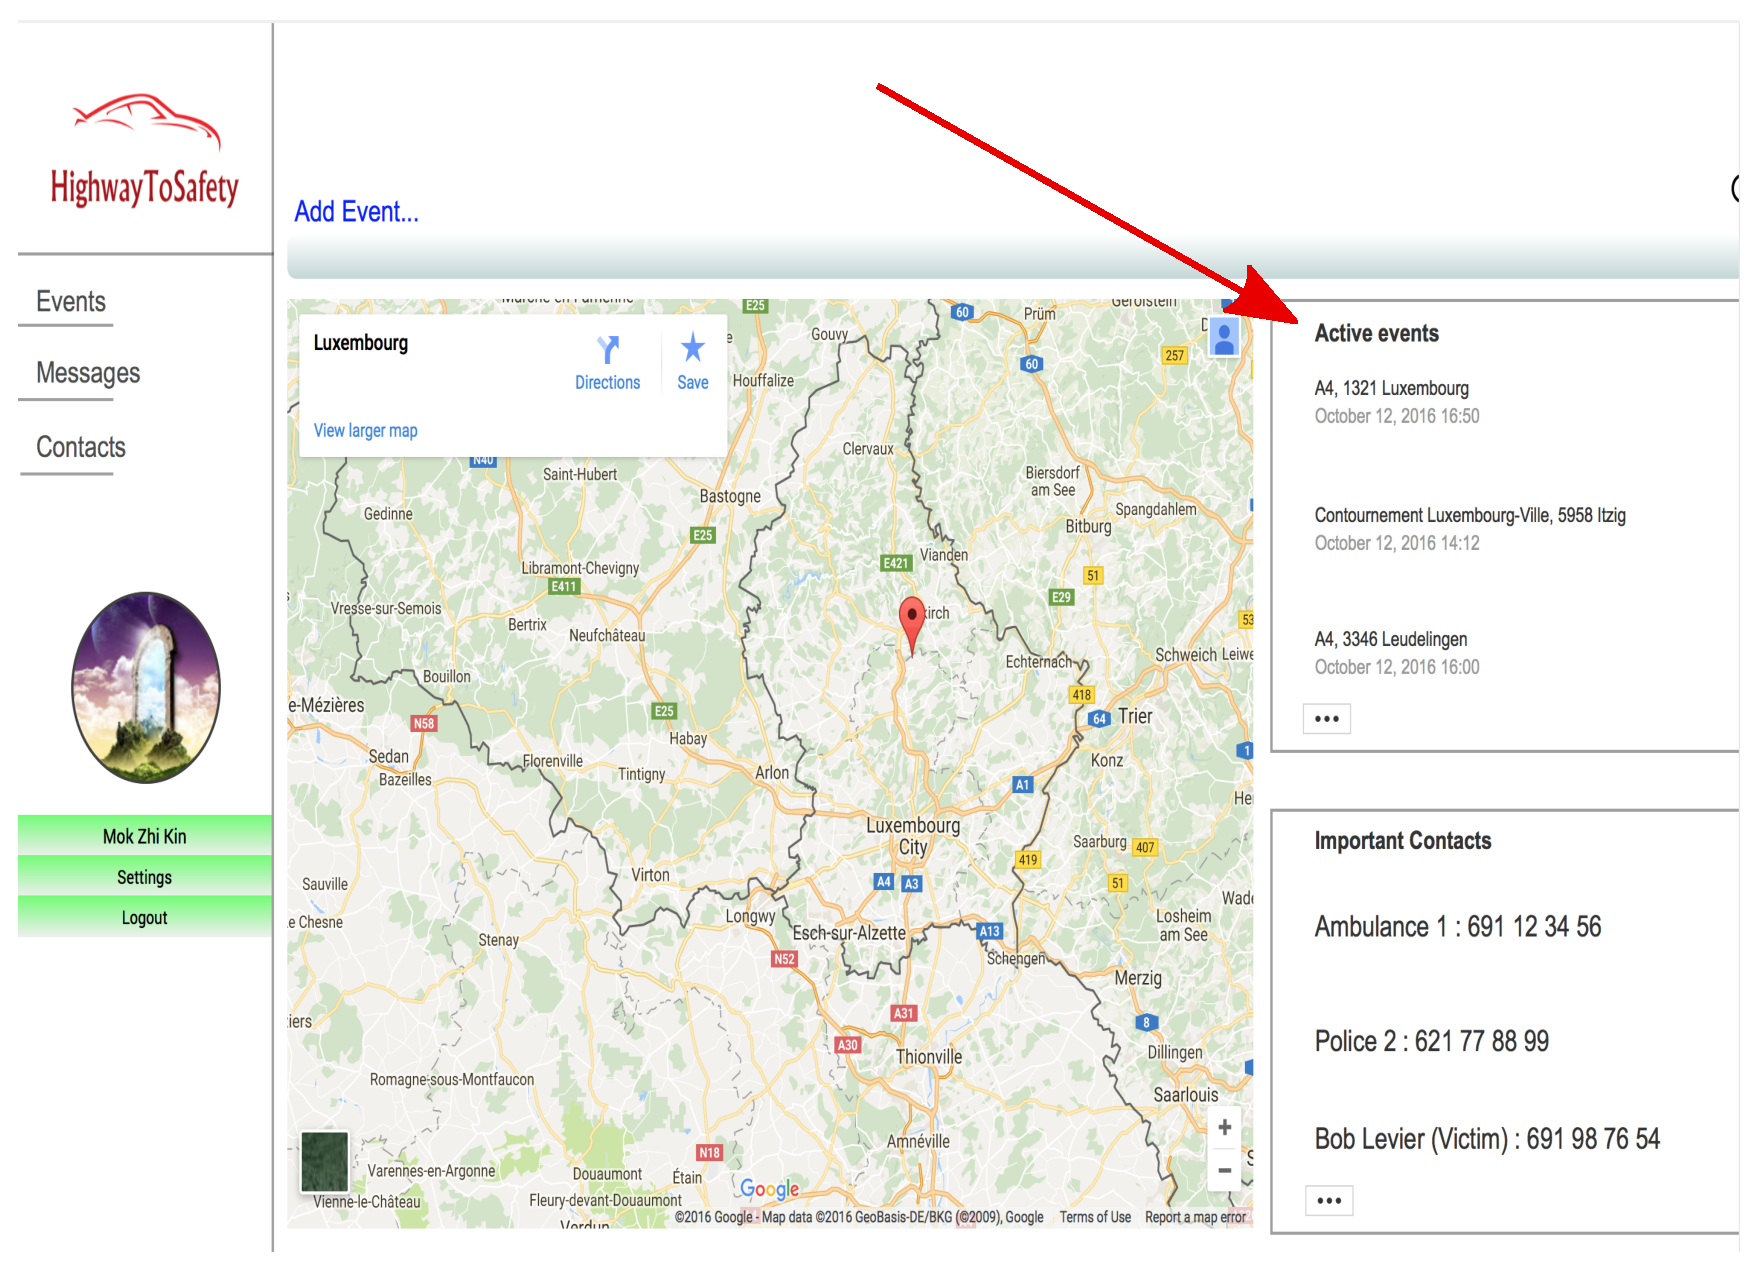
\includegraphics[width=0.9\textwidth]{Active_events.eps}
\end{figure}
\end{minipage}



\section{Send a message to the Emergency Central}
\label{operation:MyOperation}
The fireman coordinator writes a message and then sends it to the central
coordinator, either by typing in text or by using the preprogrammed macros.

\begin{description}

\item \textbf{Parameters:} Typed-in text, Quantity of assistance.
\item \textbf{Precondition:} The fireman coordinator is logged into the Ipad
app.
\item \textbf{Post-condition:} A new message has been send to the central
coordinator. 
\item \textbf{Output messages:}
\begin{enumerate}
  \item The fireman coordinator sees in the chat log that the message went out.
  \item The message displays in the GUI of the central coordinator.
\end{enumerate}

\item \textbf{Triggering:}
\begin{enumerate}
  \item From the main menu of the Ipad App click on the “Chat” button.
  \item In the chat window, you can choose rather to use the preprogrammed
  macros or to type in text manually.
  \item To use the macros you have to choose what kind of assistance you need
  (Ambulance, Police, Firetruck) and select the quantity you need, then you
  press the button with the wished assistance.
  \item To write customized messages, you can use the input field which says
  “write here\ldots”.
\end{enumerate}
\end{description}

 
\subsection{Send a message to the Emergency Central example}
The fireman coordinator wants to send a message to inform the central
coordinator that they need 3 more policemen. The fireman coordinator clicks on
the “Chat” button to enter the chat window (see Fig. 4.3). The fireman
coordinator sets the value next to the police logo to 3 and clicks on the
police logo(see Fig.4.4).
After the successfull sending of the message, the message
appears in the chat log of the fireman coordinator and on the GUI of the central
coordinator under the “Messages” window (see Fig.4.4).

\begin{minipage}{1.0\textwidth}
\begin{figure}[H]
\caption{Main menu of Ipad app}
\includegraphics[width=0.9\textwidth]{IpadAppHome1.eps}
\end{figure}
\end{minipage}

\begin{minipage}{1.0\textwidth}
\begin{figure}[H]
\caption{Chat menu of Ipad app}
\includegraphics[width=0.9\textwidth]{Chat_Example.eps}
\end{figure}
\end{minipage}

\section{Update Status on Ipad Application}
\label{operation:MyOperation}
The coordinator, who uses the Ipad, updates his status to inform the system if
his team is stil in “Staion”, “In transit” or already “Arrived”

\begin{description}

\item \textbf{Parameters:} Status input.
\item \textbf{Precondition:} The coordinator's Team is in a certain status and
the coordinator is logged into the Ipad app.
\item \textbf{Post-condition:} The coordinator's Team is in another status then
in the Precondition.
\item \textbf{Output messages:} The central coordinator of the emergency central
receives a message that the status of the coordinator's team has been updated in
the system and the changes are displayed in his GUI.

\item \textbf{Triggering:} 
\begin{enumerate}
  \item From the main menu of the Ipad App click on the “Map” button.
  \item In the map window click on the menu underneath the “Status:” label and
  select the status you want to update to.
\end{enumerate}
\end{description}

 
\subsection{Update Status on Ipad Application example}
In the main menu of the Ipad app, the coordinator of a team clicks on the “Map”
button to open the map window (see Fig. 4.3). In the map window the user clicks
on the menu underneath the “Status:” label and selects the status “Arrived” to tell the system that the
team has arrived on the accidesnt's location (see Fig. 3.2).

\section{Update Map on Ipad Application}
\label{operation:MyOperation}
The coordinator, who uses the Ipad, updates the map to get the newest
information on his map, like traffic information, accident location information or location
of other parties like ambulance, tow-truck, police.

\begin{description}

\item \textbf{Parameters:} 
\item \textbf{Precondition:} The Ipad user is on the “Map” window of
the Ipad app.
\item \textbf{Post-condition:} The map is updated and shows all the new
information.
\item \textbf{Output messages:} The map of the “Map” window changes.


\item \textbf{Triggering:}
\begin{enumerate}
  \item From the main menu of the Ipad App click on the “Map” button.
  \item Click on the “Update” button.
\end{enumerate}
 

\end{description}

 
\subsection{Update Map on Ipad Application example}
In the main menu of the Ipad app, the user clicks on the “Map” button to open
the map window (see Fig. 4.3). In the map window the user clicks on the “Update”
button to update the map. After a few seconds the updated map is displayed and all the
newest information is shown.

\newpage

% Error messages and problem resolution

\chapter{Error messages and problem resolutions}
\label{chap:error_messages}

All known problems in using the software should be listed and explained in
details using the structure presented below.

Contact information for reporting any problems (either with the software or
this document) should be clearly indicated


\section{Error message 1}

\subsection{Problem identification}
A description explaining the meaning of the faced problem.

\subsection{Probable cause}
A description explaining the reasons why such a problem has been raised.

\subsection{Corrective actions}
Describe the required steps the actor should take to recover from such situation.

\newpage

%APPENDICES
\appendix
\chapter{Title of the appendix 1}
\label{chap:appendix1}
%Reducing the spacing from the title


%Here you write the context of the appendix, structuring such content in
%sections, sub-sections and sub-sub-sections, if needed.

%An example of appendix is the flat presentation of all the graphical user
% interface screens.
%Each screen can be presented (identification symbol and description) and
% screens transition graph can be given.


\section{My Section}
\label{sec:appendix1_mySection}
%Description of the section.



\subsection{My subSection}

\subsubsection{My subSubSection}


 

	

\newpage

   
%GLOSSARY
%Uncomment the line below if you want to print all glossaries no matter if they
% appear in the document
%\glsaddall
\printglossaries
\newpage


%BIBLIOGRAPHY
\cleardoublepage 
\bibliographystyle{./../lu.uni.lassy.excalibur.standard.report.libraries/styles/lncs} 
\bibliography{./../lu.uni.lassy.excalibur.standard.report.libraries/defs/references/messir,doc/bibliography/user-manual}
\label{sec:references}

\end{document}
